\chapter{The Neutrino Maxing Angle \texorpdfstring{$\theta_{13}$}{theta13}}

\section{Overview of Neutrino Physics}

\subsection{The Postulation and Discovery of Neutrinos}
On December 4 1930, in an open letter addressed to "Dear Radioactive Ladies and Gentlemen" attempting to salvage one of the most fundamental principles in physics, energy conservation, W. Pauli postulated a neutral weakly interacting particle which is later dubbed \emph{neutrino} and opened up neutrino physics.

In nuclear beta decays, the electrons emitted by the unstable nuclei have a continuous spectrum instead of a sharp peak, which would violate energy conservation if beta decays were 2-body decay. There are two proposed solutions to this problem. N. Bohr proposed that energy conservation was only valid statistically. On the other hand, Pauli noticed that if the nuclear beta decay were a 2-body decay, not only the energy conservation but the angular momentum conservation was violated since the daughter nucleus was observed to have the same integer or fractional spin as the mother nucleus. This led Pauli to  postulate the other solution: a third undetected spin-$\frac{1}{2}$ particle takes away the missing energy. In 1934, E. Fermi formulated the first theory of weak interactions, the Fermi theory of beta decay.

Since neutrinos barely interact with matter, a direct detection would require a very strong source, which supposedly makes the nuclear power plants a very good candidate. The existence of neutrino was demonstrated by C. L. Cowan and F. Reines~\cite{Cowan1956} in their 1956 experiment at Savannah River nuclear power plant. The detection reaction they utilized is the inverse beta decay,
\begin{equation}
	\bar{\nu}_e+p\rightarrow e^++n
\end{equation}
which turns the antineutrinos from the reactor cores into a positron and a neutron, which are detectable. Cowan and Reines used a water tank filled with water with dissolved CdCl$_2$ as the target. Cadmium is a strong neutron absorber and is commonly used in control rods for nuclear reactors. Sandwiching the water tank were scintillators and photomultiplier tubes (PMTs). Immediately after the inverse beta decay reaction, the positron annihilates with an electron, generating 511 keV photons which go through scinllators and are detected by PMTs. The neutron propagates through water, loses its kinetic energy through collision until it gets to thermal energy at which Cadmium has large neutron capture cross section and gets captured by Cadmium. The excited Cadmium then de-excites and emits gamma rays which in turn are detected by the scintillators and PMTs. The time between the prompt positron annihilation and the delayed neutron capture is within 10 $\mu$s~\cite{Cowan1956}. Through this prompt-delayed coincidence the background is reduced. Neutrino detection by this prompt-delayed coincidence is a model for later neutrino experiments.

\subsection{Solar Neutrino Problem and Neutrino Oscillation}
Neutrino oscillation was first proposed in 1957 by B. Pontecorvo~\cite{Pontecorvo1957} with the neutral kaon $K^0\leftrightarrow\bar{K}^0$ strangeness oscillation as the prototype. It was found that after some time of propagation in space $\bar{K}^0$ can emerge from an initially pure $K^0$ beam and back to $\bar{K}^0$. Since the strangeness content of $\bar{K}^0$ is different from that of $K^0$, the phenomenon is called strangeness oscillation. Although $K^0$ and $\bar{K}^0$ are produced via the strong force, they decay weakly. There are two weak eigenstates, $K_L$ and $K_S$, corresponding to very different lifetime with subscripts meaning long and short, respectively; the strong eigenstates can be written as linear combinations of the weak eigenstates. The oscillation is caused by the slight difference in their masses. By measuring the appearance probability of $\bar{K}^0$ in the $K^0$ as a function of time, one can obtain the mass splitting of $K_L$ and $K_S$~\cite{Carithers1975}~\cite{Das2003}.

In the late 1960s the Homestake Experiment, directed by R. Davis, measured the neutrino flux from the Sun and found the flux was only about one-third of the prediction from the Standard Solar Model~\cite{Bahcall2003}. This discrepancy is known as the Solar Neutrino Problem. In 1962, the muon neutrino was discovered~\cite{Danby1962}, signaling the existence of more than one species of neutrino. In 1969, as an attempt to solve the solar neutrino problem, a theory of massive neutrinos~\cite{Gribov1969} was proposed in which neutrinos oscillate between 2 different flavors as they propagate in space. The existence of the third kind of neutrino, $\nu_{\tau}$ was immediately postulated when a third lepton, the $\tau$, was discovered in 1975, and the discovery of $\nu_{\tau}$ had to wait until July 2000~\cite{Donut2001}.

The first definitive evidence of neutrino oscillation came in 1998. Super-Kamiokande published its observation~\cite{Fukuda1998} that fewer $\nu_{\mu}$ come from the bottom of the detector than from the top by measuring the muons produced by charge current interactions which is consistent with the $\nu_{\mu}\leftrightarrow \nu_{\tau}$ oscillation hypothesis because neutrinos from the bottom of the detector have to travel through the earth to reach the detector. In 2001 the Sudbury Neutrino Observatory (SNO) in Canada confirmed the solar neutrino oscillation. The weak interaction is mediated by the exchange of weak bosons. Interactions involving the exchange of charged bosons are called charged current interactions, while those involving the exchange of neutral bozons are called neutral current interactions. SNO can measure the neutrino interactions through charged current or neutral current interactions. Charged current interactions are only sensitive to $\nu_e$ while neutral current interactions are sensitive to all flavors. The neutrino flux inferred from the charged current events is about one-third of the flux from neutral current events, confirming the solar neutrino oscillation.

These oscillation results from solar, atmospheric, accelerator, and long baseline reactor neutrino experiments can be explained very well by the model of three neutrino mixing. In this model, neutrinos interact or are produced in their weak eigenstates, which are not their mass eigenstates. In fact, the weak eigenstates are linear combinations of their mass eigenstates with definite masses. To be more specific, weak eigenstates can be obtained from mass eigenstates by a unitary transformation. As a neutrino propagates through space, the quantum mechanical phases of the three mass states evolve at slightly different rates due to the slight differences in the neutrino masses. This results in a changing mixture of mass states as the neutrino travels, but a different mixture of mass states corresponds to a different mixture of flavor states. The consequence is that after a flavor eigenstate is allowed to freely propagate in the space for some time, the mass eigenstate content changes. When the flavor is determined later on, the probability that it stays in the same original flavor is not 1, and there is some finite probability that it changes to other flavors. Since the neutrino flavor changes back and forth between different flavors when it propagates, the phenomenon is called neutrino oscillation. By studying the oscillation phenomenon, important parameters related to the transformation matrix or the states can be measured (see Section~\ref{sec:oscillation_theory}). There are three mixing angles $\theta_{12}$, $\theta_{23}$, $\theta_{13}$, and a CP-violating phase $\delta_{CP}$ pertaining to the mixing matrix. There are also three masses of the three mass eigenstates $m_1$, $m_2$, and $m_3$. However, most neutrino oscillation experiments are only sensitive to the mass squared splitting, $\Delta m_{ij}^2\equiv m_i^2-m_j^2$. By the time the Daya Bay neutrino experiment was designed, there was already precise knowledge in $\Delta m^2_{21}$, the absolute value of $\Delta m^2_{31}\approx \Delta m^2_{32}$, and the values of two mixing angles, $\theta_{12}$ and $\theta_{23}$. Measuring $\theta_{13}$ is important in the sense that $\delta_{CP}$ shows up in the mixing matrix along with the term involving $\theta_{13}$, and $\delta_{CP}$ may shed some light on the CP violation in the lepton sector. The Daya Bay neutrino experiment was designed to precisely measure $\theta_{13}$, and in 2012, Daya Bay collaboration published a paper on the 5.2$\sigma$ discovery of a non-zero $\theta_{13}$. The value of $\theta_{13}$ turned out to be relatively large, making the future experiments relatively easier.

\section{Neutrino Oscillation and \texorpdfstring{$\theta_{13}$}{theta13}}\label{sec:oscillation_theory}

\subsection{Neutrino Mixing and Neutrino Oscillation}
According to the Standard Model of Particle Physics, there are 3 flavors of neutrinos, namely, $\nu_e$, $\nu_\mu$, and $\nu_\tau$. These are the eigenstates when neutrinos take part in weak interactions~\cite{Olive2014}. However, these are not the eigenstates when neutrinos propagate freely in space. Since neutrinos have minute but nonzero mass, there are 3 mass eigenstates and the relation between flavor and mass eigenstates can be written as
\begin{equation}
\left( \begin{array}{c} \nu_e \\ \nu_\mu \\ \nu_\tau \end{array} \right)
=
\begin{pmatrix}
U_{e1} & U_{e2} & U_{e3} \\
U_{\mu1} & U_{\mu2} & U_{\mu3} \\
U_{\tau1} & U_{\tau2} & U_{\tau3}
\end{pmatrix}
\left( \begin{array}{c} \nu_1 \\ \nu_2 \\ \nu_3 \end{array} \right)
\end{equation}

The unitary matrix $[U_{lj}]$ is called PMNS matrix named after physicists B. Pontecorvo, Z. Maki, M. Nakagawa, and S. Sakata and can be parametrized by~\cite{Valle2006}

\allowdisplaybreaks
%\begin{align}
%U_{PMNS}=
%\begin{pmatrix}
%c_{12}c_{13} & s_{12}c_{13} & s_{13}e^{-i\delta} \\
%-s_{12}c_{23}-c_{12}s_{23}s_{13}e^{-i\delta} & c_{12}c_{23}-s_{12}s_{23}s_{13}e^{-i\delta} & s_{23}c_{13} \\
%s_{12}s_{23}-c_{12}c_{23}s_{13}e^{-i\delta} & -c_{12}s_{23}-s_{12}c_{23}s_{13}e^{-i\delta} & c_{23}c_{13}
%\end{pmatrix}
%\begin{pmatrix}
%e^{i\phi_1} & 0 & 0 \\
%0 & e^{i\phi_2} & 0 \\
%0 & 0 & 1
%\end{pmatrix}
%\end{align}
\begin{align}
U_{PMNS}=
\begin{pmatrix}
c_{12}c_{13} & s_{12}c_{13} & s_{13}e^{-i\delta} \\
-s_{12}c_{23}-c_{12}s_{23}s_{13}e^{-i\delta} & c_{12}c_{23}-s_{12}s_{23}s_{13}e^{-i\delta} & s_{23}c_{13} \\
s_{12}s_{23}-c_{12}c_{23}s_{13}e^{-i\delta} & -c_{12}s_{23}-s_{12}c_{23}s_{13}e^{-i\delta} & c_{23}c_{13}
\end{pmatrix}
\end{align}
where $c_{ij}=\cos\theta_{ij}$, $s_{ij}=\sin\theta_{ij}$.

If an electron antineutrino $\bar{\nu}_e$ is produced at the source and propagates in space, at a distance $L$ away from the source the survival probability, i.e. the probability that the neutrino doesn't change to other flavors, is
\allowdisplaybreaks
\begin{align}
P(\bar{\nu}_e\rightarrow\bar{\nu}_e)=1-c^4_{13}\sin^22\theta_{12}\sin^2\Delta_{21}-c^2_{12}\sin^22\theta_{13}\sin^2\Delta_{31}-s^2_{12}\sin^22\theta_{13}\sin^2\Delta_{32}
\end{align}
where
\begin{eqnarray}
	\Delta_{jk} & \equiv & 1267\Delta m^2_{jk}(eV^2)\times \frac{L(km)}{E(MeV)} \\
	\Delta m^2_{jk} & \equiv & m^2_j-m^2_k
\end{eqnarray}

Among the three mixing angles, $\theta_{13}$ was the only unknown parameter~\cite{dybtdr}, and the goal of Daya Bay experiment at the time of the proposal was to measure $\sin^22\theta_{13}$ with $0.01$ sensitivity at $90\%$ confidence level.


\subsection{Neutrino Flux and Energy Spectrum}

Nuclear power is generated by fission reactions mainly from 4 kinds of isotopes, namely $^{235}$U, $^{239}$Pu, $^{238}$U, and $^{241}$Pu~\cite{Kopeikin2004}. The fission products undergo beta decay and generate neutrinos as a by-product. Each fission reaction on average produces about 6 neutrinos. The detailed neutrino flux and energy spectrum at a particular time depend on the relative abundances of the isotopes, the total reactor thermal power, the fission rate of individual isotopes, and the spectrum of the individual isotopes. The number of neutrinos released by the reactor per unit time is
\begin{equation} \label{eq:neutrino_flux}
  \phi(E)=\frac{W_{th}}{\sum\limits_{i=1}^4f_ie_i}\sum\limits_{i=1}^4f_iS_i(E)
\end{equation}
where $i$ runs over the four main isotopes, $W_{th}$ is the total thermal power, $f_i$ is the fission fraction, $e_i$ is the fission energy release, and $S_i(E)$ is the neutrino energy spectrum.

The fission fraction of each isotope and the total thermal power are monitored and the weekly averaged numbers are offered by the nuclear power plant. $e_i$ is the part of the fission energy that converts into heat. Typical values at the midpoint of the reactor operation period is given in Table~\ref{table:thermal_fission_energy}~\cite{Kopeikin2004}.
\begin{table}
	\centering
	\begin{tabular}{|c|c|}
	\hline
	isotope & $e_i$ (MeV/fission) \\
	\hline
	$^{235}$U & 201.92 ± 0.46 \\
	$^{238}$U & 205.52 ± 0.96 \\
	$^{239}$Pu & 209.99 ± 0.60 \\
	$^{241}$Pu & 213.60 ± 0.65 \\
	\hline
	\end{tabular}
	\caption{Typical thermal fission energy $e_i$ at the midpoint of the reactor operation period.}
	\label{table:thermal_fission_energy}
\end{table}

The antineutrino spectra $S_i(E)$ can be calculated from measured beta spectra. A three parameter parameterization was done by Vogel and Engel~\cite{Vogel1989}. Figure~\ref{figure:isotope_antineutrino_spectra} shows the spectra of the four dominant isotopes. $^{238}$U produces the most antineutrinos per fission while $^{239}$Pu produces the least.
\begin{figure}
	\centering
	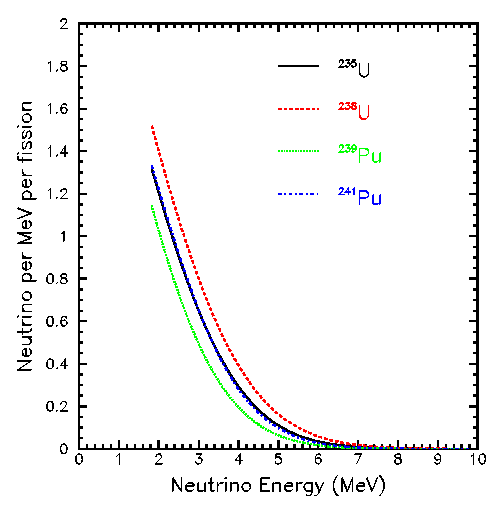
\includegraphics[width=.5\textwidth]{figures/chap2/isotope_antineutrino_spectra.eps}
	\caption{Calculated antineutrinos spectra for each dominant isotope.}
	\label{figure:isotope_antineutrino_spectra}
\end{figure}


\subsection{\texorpdfstring{$\bar{\nu}_e$}{Electron Antineutrino} Detection}
\label{sec:IBD}
Daya Bay utilizes the renowned Cowan–Reines method of prompt-delayed coincidence to detect $\bar{\nu}_e$. The reaction involved in this method is the inverse beta decay (IBD),
\begin{equation}
	\bar{\nu}_e+p\longrightarrow e^++n
\end{equation}
The positron is quickly annihilated by an electron, and photons are released which constitute the prompt signal. The neutron propagates in the target medium, slows down mainly by collisions with protons, and finally gets captured by some nucleus which in turn de-excites and releases photons constituting the delayed signal. Such prompt-delayed coincidence forms a very definitive $\bar{\nu}_e$ signature and greatly suppresses backgrounds.

The antineutrino event rate is given by
\begin{equation}
	R=\int \epsilon(E)P_{\bar{\nu}_e\rightarrow\bar{\nu}_e}(L,E)\frac{N_p\sigma(E)}{4\pi L^2}\phi(E)dE
\end{equation}
where $\epsilon$ is the antineutrino detection efficiency, $P_{\bar{\nu}_e\rightarrow\bar{\nu}_e}$ is the antineutrino survival probability, $N_p$ is the number of free protons in the form of hydrogen in the detector, $\sigma$ is the IBD total cross section, $L$ is the distance from the reactor core to the detector, and $\phi$ is the number of released antineutrinos per unit time given in Eq.~\ref{eq:neutrino_flux}.

$P_{\bar{\nu}_e\rightarrow\bar{\nu}_e}$ depends on $\sin^22\theta_{13}$ which we want to infer from the measured IBD rates. $\epsilon$, $N_p$ and $L$ are measured by auxiliary methods and instruments which will be detailed later. The total cross section of the IBD reaction in the limit of infinite nucleon mass can be written as~\cite{Vogel1999}
\begin{equation}
	\sigma^{(0)}_{tot}=0.0952\times 10^{-42} \left( \frac{E^{(0)}_ep^{(0)}_e}{1 MeV^2}\right) cm^2
\end{equation}
where $E^{(0)}_e$ and $p^{(0)}_e$ are the energy and momentum of the positron, respectively. The next-to-leading order term in $1/M$, the inverse nucleon mass, is nonnegligible. The total cross section to first order in $1/M$ is shown in Figure~\ref{fig:IBD_total_cross_section} and is adopted in Daya Bay's $\theta_{13}$ analysis.
\begin{figure}
	\centering
	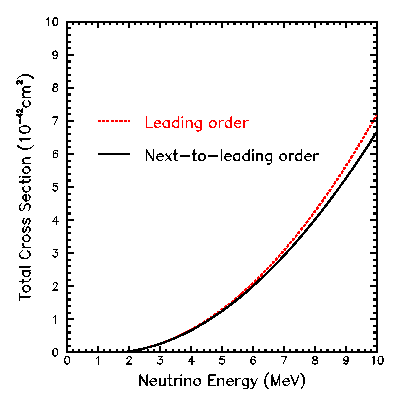
\includegraphics[width=.4\textwidth]{figures/chap2/IBD_total_cross_section.eps}
	\caption{The IBD total cross section calculated to the leading order and next-to-leading order terms.}
	\label{fig:IBD_total_cross_section}
\end{figure}
Combining the average neutrino flux with the IBD total cross section, the expected measured neutrino energy spectrum is shown in Figure~\ref{fig:IBD_rate}.
\begin{figure}
	\centering
	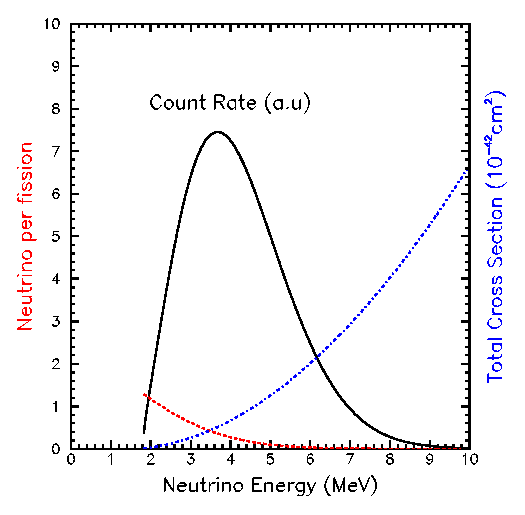
\includegraphics[width=.4\textwidth]{figures/chap2/IBD_rate.eps}
	\caption{The average neutrino flux, the IBD total cross section and the measured neutrino energy spectrum}
	\label{fig:IBD_rate}
\end{figure}


%\subsection{\texorpdfstring{$\theta_{13}$}{Theta13} Analysis and Results}
%The Daya Bay experiment completed 6 antineutrino detector installation in December 2011 and started physics data taking since December 24, 2011. With only barely 2 months of data, Daya Bay showed that $\theta_{13}$ is nonzero with a significance of 5.2 standard deviation and measured $\sin^2{2\theta_{13}}=0.092 \pm 0.016(\text{stat.}) \pm 0.005(\text{syst.})$~\cite{dyb2012_01}. In the following sections details in rate only analysis will be presented as well as the results.
%
%
%\subsubsection{Antineutrino Candidate Selection}
%A Daya Bay antineutrino signal is identified as a pair of prompt-delayed coincidence of triggers. The prompt signal is from the gammas emitted in the electron-positron annihilation process. The energy spectrum of the prompt signal therefore carries the neutrino energy information. Suppose $m_x$, $K_x$, $E_x$ represent the mass, kinetic energy and total energy of particle $x$. From energy conservation of the IBD reaction, we have
%\begin{equation}
%	E_{\bar{\nu}_e}+E_p=E_{e^+}+E_n
%\end{equation}
%The target protons are non-relativistic, $E_p\approx m_p$. Since the positron has a mass much smaller than the neutron, the neutron typically carries only 10-100 keV kinetic energy, which is negligible in the IBD energy scale. The equation becomes
%\begin{equation}
%	E_{\bar{\nu}_e}\approx K_{e^+}+\underbrace{(m_n-m_p)+m_{e^+}}_\text{1.8 MeV}
%\end{equation}
%The equation clearly shows the IBD energy threshold of 1.8 MeV. The measured prompt energy $E_{prompt}$ is the positron kinetic energy plus the annihilation energy $2\times0.511\approx 1.0$ MeV, therefore
%\begin{equation}\label{eq:nu_prompt_relation}
%	E_{\bar{\nu}_e}\approx E_{prompt}+0.8\text{ MeV}
%\end{equation}
%By referring to Figure~\ref{fig:IBD_rate} and Equation~\ref{eq:nu_prompt_relation} and take into account the smearing due to the detector energy resolution, the prompt energy cut is determined to be
%\paragraph{prompt energy cut:}
%\begin{equation}
%	0.7\text{ MeV} < E_{prompt} < 12\text{ MeV}
%\end{equation}
%
%The delayed signal comes from the de-excitation gammas from the neutron capture on $Gd$. Two $Gd$ isotopes contribute to the neutron capture process. $^{155}Gd$ has an energy of 8.536 MeV while $^{157}Gd$ is 7.937 MeV. The delayed energy cut is thus
%\paragraph{delayed energy cut:}
%\begin{equation}
%	6\text{ MeV} < E_{delayed} < 12\text{ MeV}
%\end{equation}
%
%The capture probability of a neutron on Gd between $t$ and $t+dt$ can be written as
%\begin{equation}
%  P_{cap}(E)dt=\sigma(E) n v(E)dt
%\end{equation}
%where $E$ is the neutron energy, $\sigma(E)$ is the total neutron capture cross section, $n$ is the number density of Gd and $v(E)$ is the velocity of the neutron. Figure~\ref{fig:capture_cross_section} shows the capture cross sections for $^{155}$Gd, $^{157}$Gd, $^6$Li, $^1$H, $^{10}$B and $^{113}$Cd~\cite{Bowden2012}.
%\begin{figure}
%  \centering
%  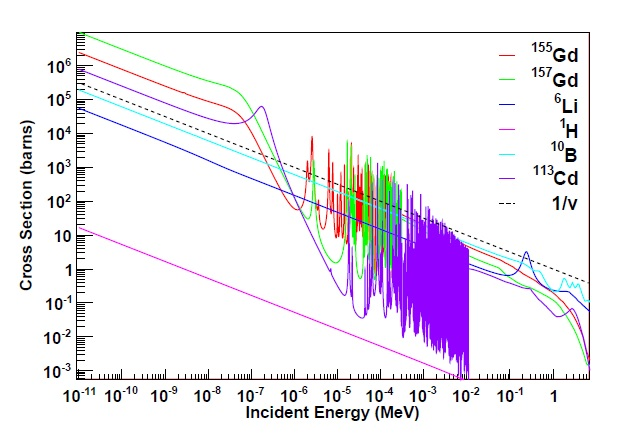
\includegraphics[width=.6\textwidth]{figures/chap2/capture_cross_section.jpg}
%  \caption{Solid lines are the capture cross sections of commonly used capture agents. The dashed line shows the $1/v$ dependence of the capture cross section.}
%  \label{fig:capture_cross_section}
%\end{figure}
%First note that the capture cross section of Gd is 5 orders of magnitude larger than the H. Besides, most elements have a cross section following $1/v$ dependence very well in the entire energy range. If we use the $\sigma(E)\sim 1/v$, $P_{cap}(E)$ is independent of energy and is a constant $\lambda$. If at time $t$, $N(t)$ neutrons survive, then $N(t+dt)=N(t)-P_{cap}dt\cdot N(t)=N(t)-\lambda dtN(t)\Rightarrow N(t)\sim e^{-\lambda t}$. In the case of $^{155}$Gd and $^{157}$Gd, however, when the energy is larger than 0.1 eV, the capture cross sections don't follow a simple $1/v$ dependence and are smaller than a $1/v$ extrapolation from below 0.1 eV. In this case $N(t)\sim e^{-\int P_{cap}dt}$ and the corresponding capture time distribution is
%\begin{equation}
%	-\frac{dN}{dt}\sim P_{cap}(t)e^{-\int P_{cap}(t)dt}
%\end{equation}
%Qualitatively speaking, the capture time distribution is greatly suppressed when $t$ is small since at the moment the neutron has a large energy which implies a small capture probability. The time for a neutron to slow down to thermal energy is called thermalization time. Figure~\ref{fig:capture_time} shows the time between the prompt and the delayed signals in antineutrino candidates.
%\begin{figure}
%	\centering
%	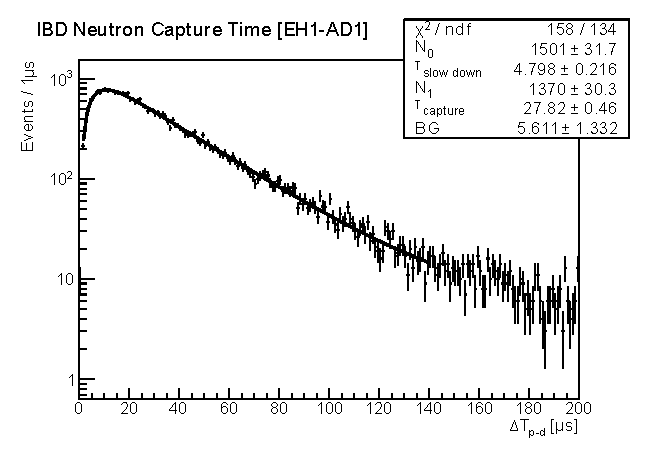
\includegraphics[width=0.6\textwidth]{figures/chap2/capture_time.eps}
%	\caption{Time between the prompt and the delayed events in antineutrino candidates.}
%	\label{fig:capture_time}
%\end{figure}
%The distribution is modeled by
%\begin{equation}
%	C(t)=-C_0e^{-t/t_0}+C_1e^{-t/t_1}+C_{bg}
%\end{equation}
%, where the first term accounts for the the thermalization process, the second term for thermal neutron capture and the third term for background. Here we conclude,
%\paragraph{capture time cut:}
%\begin{equation}
%	1\text{ }\mu\text{s}<\Delta T_{p-d}<200\text{ }\mu\text{s}
%\end{equation}
%
%
%It was found that when photomultiplier tubes are in operation, there could be electronic discharge in the PMT's base. These background events are called flasher events. At Daya Bay, about 5\% of triggers in the antineutrino detector are flasher events. The energy range of the flasher events is from the detector threshold to 100 MeV, and in the delayed signal energy range (6 MeV to 12 MeV) the flasher event rate is 0.7 Hz which is a serious background. Since the flasher events have a different timing and charge patter from physical events, a cut was easily devised to remove such background. The flasher cut is applied to every event before further selection.
%
%If a cosmic muon goes through the AD, many spallation products can be formed. Among them, the spallation neutrons and spallation $^9$Li/$^8$He can lead to prompt-delayed coincidence signal. In order to remove such backgrounds, a muon veto cut is applied which vetos the AD for 1000 $\mu s$ if the muon goes through the AD or 200 $\mu s$ if the muon goes through the water pool but not the AD.
%
%To summarize, the antineutrino candidates must pass:
%\begin{itemize}
%	\item prompt energy cut
%	\item delayed energy cut
%	\item capture time cut
%	\item flasher cut
%	\item muon veto cut
%\end{itemize}
%
%
%\subsubsection{Backgrounds}
%As mentioned in section~\ref{sec:IBD}, the signal of the Daya Bay experiment has a distinct prompt-delayed coincidence in time. However there are still background signals that can mimic such time correlation. The backgrounds of the Daya Bay neutrino experiment are:
%\paragraph{Accidental signals:} Two singles events happening to be in the correlation time window constitute the accidental background. To estimate the accidental rate, first a muon veto cut is applied to remove the non-signal time regions. Then a flasher cut is applied to assure events are physical. To obtain a true singles spectrum, the IBD events now should be removed from it. From the singles spectrum, one can estimate the prompt singles rate $R_p$ (0.7 MeV < E < 12 MeV) and the delayed singles rate $R_d$ (6 MeV < E < 12 MeV). Since the capture time window is (1 $\mu$s, 200 $\mu$s), the accidental background can then be calculated by the rates and the time interval.
%\paragraph{$^9$Li/$^8$He:} Among the various isotopes of the muon spallation products, the long lived $^9$Li/$^8$He can give events faking the IBD signal. Both $^9$Li and $^8$He have a $\beta^-$-n decay channel with a half life of 178.3 ms and 118.5 ms, respectively. To estimate the absolute number of the $^9$Li/$^8$He background, we first look for showering muons (muons deposited a large amount of energy, $>2.5$ GeV). After the showering muons, we look for the prompt-delayed coincidence. Then the timing distribution of the prompt event since the last muon can be used to estimate the number of $^9$Li/$^8$He. In KamLAND, the distribution is then fitted to the function~\cite{KamLAND_01}
%\begin{equation}
%	r(t)=\sum_i \frac{N_i}{\tau_i}e^{-(t-t_\mu)/\tau_i}+r_B
%\end{equation}
%where $i$ runs through those isotopes with similar mean lifetime, $t_\mu$ is the muon time and $N_i$, $\tau_i$ and $r_B$ are the overall number, the mean lifetime and the background, respectively. However for Daya Bay, such a simple formula is not appropriate since Daya Bay is much shallower (1200 m.w.e. at far site) than KanLAND (2700 m.w.e.). With much thicker overburden, the mean time interval between muons is 5 s, which is much larger than the mean lifetime of the isotopes considered. Daya Bay's muon rate can reach 20 Hz, i.e. 50 ms between muons. The isotopes generated by different muons "stacks" before then decay. Therefore a more sophisticated formula too account for the overlapping is required. It is shown that for shallow underground labs, the distribution can be fitted with the function~\cite{Wen2006}
%\begin{equation}
%	ttt
%\end{equation}
%
%
%
%
%
%\section{\texorpdfstring{$\theta_{13}$}{Theta13} Estimation by Rate Analysis}
%Daya Bay set out to do a precise measurement on $\theta_{13}$. More specifically, Daya Bay's physics goal is to reach a sensitivity of $0.01$ in $\sin^22\theta_{13}$ at $90\%$ confidence level. In this section the basic ideas of estimating $\theta_{13}$ from the first 8 weeks of data is presented and more details will be found in the corresponding subsection.
%
%$\theta_{13}$ can be estimated by either the inverse beta decay rate, or by the spectral shape of the neutrino energy spectrum, or in combination. The advantage of the spectral analysis is that it is sensitive to $\Delta m^2$. However since each energy bin can be seen as an independent measurement, it is computationally heavy. Here we will talk about using rate analysis to estimate the value of $\theta_{13}$.
%
%The procedures of estimating $\theta_{13}$ is as follows. First the number of IBD candidate events in a fixed amount of dataset is selected with energy, timing and muon veto cuts. Then the true number of IBD candidates is estimate by correcting for various selection cut efficiency. Besides, all backgrounds that mimic the IBD events are carefully studied and their rates are estimated. The expected number of IBD events is calculated with the knowledge of reactor flux, the IBD total cross section, the detector target mass, the baseline, and the DAQ live time.
%
%\subsection{Expected Number of Inverse Beta Decay Events}
%In the data taking period from Dec. 24 2011 to Feb. 17 2012, Daya Bay has 6 ADs installed and 6 reactor cores in operation. There are 6 measurements from the 6 ADs. Meanwhile the are 6 expected number of IBD events for each AD which are a function of $\sin^22\theta_{13}$. By measuring the number of IBD events and writing the expected number of IBD events as a function of $\theta_{13}$ one can construct a $\chi^2$ function and through minimization $\theta_{13}$ can be estimated.
%
%We will adapt a convention that the subscript $c$ runs through reactor cores and $d$ runs through antineutrino detectors. We want to know the expected number of IBD events for each AD, $T_d$. First we calculate the expected number of IBD events \emph{without} oscillation $N_d$,
%\begin{equation}\label{eq:no_osc_rate}
%	N_d=\sum\limits_{c=1}^6 \epsilon_d N^p_d \int \sigma(E)\frac{\phi_c(E)}{4\pi L_{cd}^2}dE
%\end{equation}
%where $N^p_d$ is the target number density of the $d$th detector, $E$ is the neutrino energy, $\sigma(E)$ is the inverse beta decay total cross section, $\phi_c(E)$ is the neutrino flux from core $c$ and $L_{cd}$ is the baseline from core $c$ to detector $d$. The IBD total cross section is given in \cite{Vogel1999}. The flux from core $c$ is given by Equation~\ref{eq:neutrino_flux} and depends on the instantaneous total thermal power of the reactor core which in general has a core to core difference. The detailed total thermal power is supplied by the nuclear power plant on a daily basis. The baselines are measured by GPS with a precision of 28 mm. The target masses are measure by load cells with a precision of 0.015$\%$. By putting all the information together, the expected IBD events without oscillation can be obtained. Now if we assume the fluxes from all cores have the same energy functional form and only differ in magnitude, $\phi_c=f_c\phi$, then Equation~\ref{eq:no_osc_rate} simplifies to
%\begin{equation}\label{eq:no_osc_rate_simple}
%	N_d=\sum\limits_{c=1}^6 \epsilon_d N^p_d f_c \int \sigma(E)\frac{\phi(E)}{4\pi L_{cd}^2}dE
%\end{equation}
%
%The expected number of IBD events \emph{with} oscillation $T_d$ is
%\begin{equation}\label{eq:with_osc_rate}
%	T_d=\sum\limits_{c=1}^6 \epsilon_d N^p_d f_c \int \sigma(E)P(\theta_{13},L_{cd},E)\frac{\phi(E)}{4\pi L_{cd}^2}dE
%\end{equation}
%The only difference from Equation~\ref{eq:no_osc_rate_simple} is the insertion of the neutrino survival probability, which is given by
%\begin{equation}\label{eq:sur_prob_approx}
%	P(\theta_{13},L_{cd},E)=1-\sin^22\theta_{13}\sin^2(1.267\Delta m_{32}^2L_{cd}/E)
%\end{equation}
%Here we have used $\Delta m_{31}^2=2.32^{+0.12}_{-0.08}\times 10^{-3} eV^2\approx \Delta m_{32}^2$ and kept only the leading term at Daya Bay's baseline. Substituting Equation~\ref{eq:sur_prob_approx} back to Equation~\ref{eq:with_osc_rate}, we have
%\begin{equation}\label{eq:with_osc_rate_2}
%	T_d=N_d-\sin^22\theta_{13}\frac{N^p_d}{4\pi}\sum\limits_{c}\frac{f_c}{L_{cd}^2}\int\sigma\sin^2\left(\frac{1.267\Delta m_{32}^2L_{cd}}{E}\right)\phi dE
%\end{equation}
%If we define weight by
%\begin{equation}\label{eq:omega}
%	\omega_{cd}=\frac{f_c/L_{cd}^2}{\sum\limits_{c} f_c/L_{cd}^2}
%\end{equation}
%and oscillation factor by
%\begin{equation}\label{eq:Delta}
%	\Delta_{cd}=\frac{\int\sigma\sin^2\left(\frac{1.267\Delta m_{32}^2L_{cd}}{E}\right)\phi dE}{\int\sigma\phi dE}
%\end{equation}
%and divide Equation~\ref{eq:with_osc_rate_2} by $N_d$, we arrive at the result
%\begin{equation}\label{eq:with_osc_rate_final}
%	\frac{T_d}{N_d}=1-\sin^22\theta_{13}\sum\limits_{c}\omega_{cd}\Delta_{cd}
%\end{equation}
%$N_d$ was calculated previously, and $\omega_{cd}$ and $\Delta_{cd}$ can also be calculated from available data, so $T_d$ can be expressed as a function of the one parameter to be estimated, namely $\sin^22\theta_{13}$. If we call the second term in Equation~\ref{eq:with_osc_rate_final} oscillation deficit, the result in this data taking period is shown in Table~\ref{table:ocs_deficit}.
%\begin{table}
%  \centering
%	\begin{tabular}{|c|c|c|c|c|c|}
%		\hline
%		AD1 & AD2 & AD3 & AD4 & AD5 & AD6 \\
%		\hline
%		0.148$\sin^22\theta_{13}$ & 0.145$\sin^22\theta_{13}$ & 0.20$\sin^22\theta_{13}$ & 0.77$\sin^22\theta_{13}$ & 0.77$\sin^22\theta_{13}$ & 0.77$\sin^22\theta_{13}$ \\
%		\hline
%	\end{tabular}
%	\caption{Oscillation deficit for six ADs}
%	\label{table:ocs_deficit}
%\end{table}
%
%
%\begin{table}
%	\centering
%	\begin{tabular}{|c|c|c|c|c|c|c|}
%		\hline
%		detector & AD1 & AD2 & AD3 & AD4 & AD5 & AD6 \\
%		\hline
%		\hline
%		IBD candidates & 28935 & 28975 & 22466 & 3528 & 3436 & 3452 \\
%		\hline
%		total backgrounds & 556.19 & 441 & 358 & 145 & 148 & 139 \\
%		\hline
%	\end{tabular}
%	\caption{IBD analysis results}
%	\label{table:IBD}
%\end{table}
%
%\begin{table}
%	\centering
%	\begin{tabular}{|c|c|c|c|c|c|c|}
%	\hline
%	detector & AD1 & AD2 & AD3 & AD4 & AD5 & AD6 \\
%	\hline
%	\hline
%	measured IBD number & 28379 & 28418 & 22034 & 3354.3 & 3260.4 & 3286.1 \\
%	\hline
%	predicted IBD number & 28083 & 28522 & 21895 & 3496.3 & 3502.6 & 3466.3 \\
%	\hline
%	measured/predicted & 101.0$\%$ & 99.6$\%$ & 100.6$\%$ & 95.9$\%$ & 93.9$\%$ & 94.8$\%$ \\
%	\hline
%	\end{tabular}
%	\caption{ratio of number of measured and predicted IBD events.}
%	\label{table:IBD_ratio}
%\end{table}
%
%Table~\ref{table:IBD} shows the analysis results of number of IBD candidates and total backgrounds. Table~\ref{table:IBD_ratio} shows the number of measured IBD events with background subtracted, the number of predicted IBD events \emph{without} oscillation, and the ratio of the two numbers. A heuristic way to estimate $\sin^22\theta_{13}$ is to take the ratios from any 2 ADs, form the difference, and compare with the same difference with numbers taken from Table~\ref{table:ocs_deficit}. For example if we take AD1 and AD6, we have $(0.77-0.148)\sin^22\theta_{13}=101\%-94.8\%$, or $\sin^22\theta_{13}=0.099$.
%
%Another way to estimate $\sin^22\theta_{13}$ is to use the so called "relative measurement", i.e. by forming the ratio of two IBD rates registered by two different detectors. By this way we don't have to rely on the absolute calculation of $N_d$ and the systematic uncertainties concerning to the absolute reactor flux will cancel when forming the ratio. To start with, we take one of the far site AD and denote quantities concerning to the AD by subscript $d=F$. Meanwhile we take a near site AD and denote quantities with subscript $d=N$. The ratio of the two estimated rates is
%\begin{equation}\label{eq:relative1}
%	\frac{T_F}{T_N}=\frac{\epsilon_F}{\epsilon_N}\frac{\sum\limits_c \frac{N^p_df_c}{4\pi L^2_{cF}}\int\sigma\phi P_{cF}dE}{\sum\limits_c \frac{N^p_df_c}{4\pi L^2_{cN}}\int\sigma\phi P_{cN}dE}
%\end{equation}
%If we further assume that the target mass $N^p_d$ is the same across detectors, Equation~\ref{eq:relative1} simplfies to
%\begin{equation}
%	\frac{T_F}{T_N}=\frac{\epsilon_F}{\epsilon_N}\frac{\sum\limits_c \frac{f_c}{L^2_{cF}}\int\sigma\phi P_{cF}dE}{\sum\limits_c \frac{f_c}{L^2_{cN}}\int\sigma\phi P_{cN}dE}
%\end{equation}
%Now by employing Equation~\ref{eq:sur_prob_approx},~\ref{eq:omega} and~\ref{eq:Delta}, we have
%\begin{eqnarray}
%	\frac{T_F}{T_N}&=&\frac{\epsilon_F}{\epsilon_N}\frac{\frac{1}{\bar{L}^2_F}\sum\limits_c \omega_{cF}\left( 1-\sin^22\theta_{13}\Delta_{cF} \right)}{\frac{1}{\bar{L}^2_N}\sum\limits_c \omega_{cN}\left( 1-\sin^22\theta_{13}\Delta_{cN} \right)} \\
%	&=&\frac{\epsilon_F}{\epsilon_N}\frac{\bar{L}^2_N}{\bar{L}^2_F}\frac{1-\sin^22\theta_{13}\sum\limits_c\omega_{cF}\Delta_{cF}}{1-\sin^22\theta_{13}\sum\limits_c\omega_{cN}\Delta_{cN}}
%\end{eqnarray}
%where we have defined the flux-weighted baseline $\bar{L}_d$ as
%\begin{equation}
%	\frac{1}{\bar{L}^2_d}=\sum\limits_c \frac{f_c}{L_{cd}^2}
%\end{equation}
%and used the identity $\sum\limits_c\omega_{cd}=1$ for all $d$.
%The unblinded baselines $L_{cd}$ from core $c$ to detector $d$ is tabulated in Table~\ref{table:baseline}.
%\begin{table}
%	\centering
%	\begin{tabular}{|c|c|c|c|c|c|c|}
%		\hline
%		(m) & D1 & D2 & L1 & L2 & L3 & L4 \\
%		\hline
%		AD1 & 362.3773 & 371.759 & 903.4704 & 817.1618 & 1353.622 & 1265.319 \\
%		AD2 & 357.9373 & 368.4106 & 903.3506 & 816.9001 & 1354.233 & 1265.89 \\
%		AD3 & 1332.475 & 1358.144 & 467.5708 & 489.5737 & 557.5798 & 499.2072 \\
%		AD4 & 1919.63 & 1894.335 & 1533.177 & 1533.625 & 1551.381 & 1524.937 \\
%		AD5 & 1917.516 & 1891.974 & 1534.916 & 1535.029 & 1554.764 & 1528.043 \\
%		AD6 & 1925.253 & 1899.859 & 1538.927 & 1539.465 & 1556.341 & 1530.076 \\
%		\hline
%	\end{tabular}
%	\caption{Baselines between reactor cores and ADs. D means Daya Bay power plant and L means Ling Ao power plant.}
%	\label{table:baseline}
%\end{table}
%The reactor thermal power for each reactor core is provided by the nuclear power plant in the form of daily average and is stored and readily accessed in Daya Bay's offline database. Therefore $\bar{L}_d$, $\omega_{cd}$ and $\Delta_{cd}$ can be calculated and are listed in Table~\ref{table:weighted_baseline}, Table~\ref{table:weight} and Table~\ref{table:osc_factor}.
%\begin{table}
%	\centering
%	\begin{tabular}{|c|c|c|c|c|c|c|}
%		\hline
%		detector & AD1 & AD2 & AD3 & AD4 & AD5 & AD6 \\
%		\hline
%		flux-weighted baseline (m) & 497 & 491 & 554 & 1627 & 1628 & 1632 \\
%		\hline
%	\end{tabular}
%	\caption{Flux-weighted baselines for 6 ADs.}
%	\label{table:weighted_baseline}
%\end{table}
%\begin{table}
%	\centering
%	\begin{tabular}{|c|c|c|c|c|c|c|}
%		\hline
%		 & D1 & D2 & L1 & L2 & L3 & L4 \\
%		\hline
%		AD1 & 0.417562 &0.426367 &0.0383572 &0.0539022 &0.0300287 &0.0337836 \\
%		AD2 & 0.420337 &0.426393 &0.0376817 &0.0529728 &0.0294655 &0.0331499 \\
%		AD3 & 0.0411601 &0.0425759 &0.190634 &0.20044 &0.235894 &0.289297 \\
%		AD4 & 0.140358 &0.154889 &0.125564 &0.143849 &0.215749 &0.219591 \\
%		AD5 & 0.140904 &0.155538 &0.12549 &0.143828 &0.215173 &0.219068 \\
%		AD6 & 0.140465 &0.155011 &0.125454 &0.143706 &0.215798 &0.219566 \\
%		\hline
%	\end{tabular}
%	\caption{Weight table}
%	\label{table:weight}
%\end{table}
%\begin{table}
%	\centering
%	\begin{tabular}{|c|c|c|c|c|c|c|}
%		\hline
%		 & D1 & D2 & L1 & L2 & L3 & L4 \\
%		\hline
%		AD1 & 0.0826245 &0.0855193 &0.415679 &0.352319 &0.683062 &0.639695 \\
%		AD2 & 0.0806925 &0.0840498 &0.415596 &0.35214 &0.683346 & 0.639996 \\
%		AD3 & 0.676348 &0.682713 &0.133883 &0.144174 &0.183527 &0.150169 \\
%		AD4 & 0.812616 &0.811365 &0.756031 &0.752377 &0.758721 &0.750827 \\
%		AD5 & 0.812625 &0.811305 &0.75657 &0.75282 &0.759727 &0.751819 \\
%		AD6 & 0.812577 &0.811492 &0.757804 &0.754208 &0.760193 &0.752464 \\
%		\hline
%	\end{tabular}
%	\caption{Oscillation factor}
%	\label{table:osc_factor}
%\end{table}
%\begin{table}
%	\scriptsize
%	\centering
%	\begin{tabular}{|c|c|c|c|c|c|c|}
%		\hline
%		 & AD1 & AD2 & AD3 & AD4 & AD5 & AD6 \\
%		\hline
%		IBD candidates & 28935 & 28975 & 22466 & 3528 & 3436 & 3452 \\
%		veto cut efficiency & 0.8019 & 0.7989 & 0.8363 & 0.9547 & 0.9543 & 0.9538 \\
%		Accidentals (per day) & 9.82±0.06 & 9.88±0.06 & 7.67±0.05 & 3.29±0.03 & 3.33±0.03 & 3.12±0.03 \\
%		Fast-neutron (per day) & 0.84±0.28 & 0.84±0.28 & 0.74±0.44 & 0.04±0.04 & 0.04±0.04 & 0.04±0.04 \\
%		$^9$Li/$^8$He (per AD per day) & 3.1±1.6 & 3.1±1.6 & 1.8±1.1 & 1.8±1.1 & 0.16±0.11 & 0.16±0.11 \\
%		Am-C correlated (per AD per day) & 0.2±0.2 & 0.2±0.2 & 0.2±0.2 & 0.2±0.2 & 0.2±0.2 & 0.2±0.2 \\
%		$^{13}$C($\alpha$,n)$^{16}$O background (per day) & 0.04±0.02 & 0.04±0.02 & 0.035±0.02 & 0.03±0.02 & 0.03±0.02 & 0.03±0.02 \\
%		\hline
%	\end{tabular}
%	\caption{Signal and background summary}
%	\label{table:bkg_sig}
%\end{table}





\section{\texorpdfstring{$\theta_{13}$}{Theta13} Estimation by Rate Analysis}
Daya Bay set out to do a precise measurement on $\theta_{13}$. More specifically, Daya Bay's physics goal is to reach a sensitivity of $0.01$ in $\sin^22\theta_{13}$ at $90\%$ confidence level. In this section the basic ideas of estimating $\theta_{13}$ from the first 8 weeks of data is presented and more details will be found in the corresponding subsection.

$\theta_{13}$ can be estimated by either the inverse beta decay rate, or by the spectral shape of the neutrino energy spectrum, or in combination. The advantage of the spectral analysis is that it is sensitive to $\Delta m^2$. However, since each energy bin can be seen as an independent measurement, the analysis is much more involved. Here we will talk about using rate only analysis to estimate the value of $\theta_{13}$.

The procedures of estimating $\theta_{13}$ is as follows. First the IBD candidate events in a certain fixed amount of dataset is selected with energy, timing and muon veto cuts. Then the true number of IBD candidates is estimate by correcting for various selection cut efficiency. Besides, all backgrounds that mimic the IBD events are carefully studied and their rates are estimated. The expected number of IBD events is calculated with the knowledge of reactor flux, the IBD total cross section, the detector target mass, the baseline, and the DAQ live time.

\subsection{Expected and Measured Number of Inverse Beta Decay Events}
The Daya Bay experiment started data taking on 24 December 2011 with 6 antineutrino detectors (ADs). Data taking was paused on 28 July 2012 and two new ADs were installed. Operation of the full experiment with all 8 ADs started on 19 October 2012. In this discussion we use 404 days of data acquired in the 8-AD period combined with all 217 days of data acquired in the 6-AD period. Each AD has one measurement of number of IBD events. Meanwhile for each AD, one expected, i.e., no oscillation, the number of IBD events which is a function of $\sin^22\theta_{13}$ can be calculated. By measuring the number of IBD events and writing the expected number of IBD events as a function of $\theta_{13}$, one can construct a $\chi^2$ function, and through minimization $\theta_{13}$ can be estimated.

We will adopt a convention that the subscript $c$ runs through reactor cores and $d$ runs through antineutrino detectors. We want to know the expected number of IBD events for each AD, $T_d$. First we calculate the expected number of IBD events \emph{without} oscillation $N_d$,
\begin{equation}\label{eq:no_osc_rate}
	N_d=\sum\limits_{c=1}^6 \epsilon_d N^p_d \int \sigma(E)\frac{\phi_c(E)}{4\pi L_{cd}^2}dE
\end{equation}
where $N^p_d$ is the target number density of the $d$th detector, $E$ is the neutrino energy, $\sigma(E)$ is the inverse beta decay total cross section, $\phi_c(E)$ is the neutrino flux from core $c$, and $L_{cd}$ is the baseline from core $c$ to detector $d$. The IBD total cross section is given in \cite{Vogel1999}. The flux from core $c$ is given by Equation~\ref{eq:neutrino_flux} and depends on the instantaneous total thermal power of the reactor core which in general has a core to core difference. The detailed total thermal power is supplied by the nuclear power plant on a daily basis~\cite{docdb7610}. The baselines are measured by GPS with a precision of 28 mm~\cite{dayabay2013}. The target masses are measure by load cells with a precision of 0.015$\%$. By putting all the information together, the expected IBD events without oscillation can be obtained. Now if we assume the fluxes from all cores have the same energy functional form and only differ in magnitude, $\phi_c=f_c\phi$, then Equation~\ref{eq:no_osc_rate} simplifies to
\begin{equation}\label{eq:no_osc_rate_simple}
	N_d=\sum\limits_{c=1}^6 \epsilon_d N^p_d f_c \int \sigma(E)\frac{\phi(E)}{4\pi L_{cd}^2}dE
\end{equation}

The expected number of IBD events \emph{with} oscillation $T_d$ is
\begin{equation}\label{eq:with_osc_rate}
	T_d=\sum\limits_{c=1}^6 \epsilon_d N^p_d f_c \int \sigma(E)P(\theta_{13},L_{cd},E)\frac{\phi(E)}{4\pi L_{cd}^2}dE
\end{equation}
The only difference from Equation~\ref{eq:no_osc_rate_simple} is the insertion of the neutrino survival probability, which is given by
\begin{equation}\label{eq:sur_prob_approx}
	P(\theta_{13},L_{cd},E)=1-\sin^22\theta_{13}\sin^2(1.267\Delta m_{32}^2L_{cd}/E)
\end{equation}
Here we have used $\Delta m_{31}^2=2.32^{+0.12}_{-0.08}\times 10^{-3} eV^2\approx \Delta m_{32}^2$ and kept only the leading term at Daya Bay's baseline. Substituting Equation~\ref{eq:sur_prob_approx} back to Equation~\ref{eq:with_osc_rate}, we have
\begin{equation}\label{eq:with_osc_rate_2}
	T_d=N_d-\sin^22\theta_{13}\frac{N^p_d}{4\pi}\sum\limits_{c}\frac{f_c}{L_{cd}^2}\int\sigma\sin^2\left(\frac{1.267\Delta m_{32}^2L_{cd}}{E}\right)\phi dE
\end{equation}
If we define weight by
\begin{equation}\label{eq:omega}
	\omega_{cd}=\frac{f_c/L_{cd}^2}{\sum\limits_{c} f_c/L_{cd}^2}
\end{equation}
and oscillation factor by
\begin{equation}\label{eq:Delta}
	\Delta_{cd}=\frac{\int\sigma\sin^2\left(\frac{1.267\Delta m_{32}^2L_{cd}}{E}\right)\phi dE}{\int\sigma\phi dE}
\end{equation}
and divide Equation~\ref{eq:with_osc_rate_2} by $N_d$, we arrive at the result
\begin{equation}\label{eq:with_osc_rate_final}
	\frac{T_d}{N_d}=1-\sin^22\theta_{13}\sum\limits_{c}\omega_{cd}\Delta_{cd}
\end{equation}
$N_d$ was calculated previously, and $\omega_{cd}$ and $\Delta_{cd}$ can also be calculated from available data, so $T_d$ can be expressed as a function of the one parameter to be estimated, namely $\sin^22\theta_{13}$. If we call the second term in Equation~\ref{eq:with_osc_rate_final} oscillation deficit, the result in these data taking period is shown in Table~\ref{table:ocs_deficit}.
\begin{table}
  \centering
	\begin{tabular}{|c|c|c|c|c|c|}
		\hline
		AD1 & AD2 & AD3 & AD4 & AD5 & AD6 \\
		\hline
		0.148$\sin^22\theta_{13}$ & 0.145$\sin^22\theta_{13}$ & 0.20$\sin^22\theta_{13}$ & 0.77$\sin^22\theta_{13}$ & 0.77$\sin^22\theta_{13}$ & 0.77$\sin^22\theta_{13}$ \\
		\hline
	\end{tabular}
	\caption{Oscillation deficit for six ADs}
	\label{table:ocs_deficit}
\end{table}


\begin{table}
	\centering
	\begin{tabular}{|c|c|c|c|c|c|c|}
		\hline
		detector & AD1 & AD2 & AD3 & AD4 & AD5 & AD6 \\
		\hline
		\hline
		IBD candidates & 28935 & 28975 & 22466 & 3528 & 3436 & 3452 \\
		\hline
		total backgrounds & 556.19 & 441 & 358 & 145 & 148 & 139 \\
		\hline
	\end{tabular}
	\caption{IBD analysis results}
	\label{table:IBD}
\end{table}

\begin{table}
	\centering
	\begin{tabular}{|c|c|c|c|c|c|c|}
	\hline
	detector & AD1 & AD2 & AD3 & AD4 & AD5 & AD6 \\
	\hline
	\hline
	measured IBD number & 28379 & 28418 & 22034 & 3354.3 & 3260.4 & 3286.1 \\
	\hline
	predicted IBD number & 28083 & 28522 & 21895 & 3496.3 & 3502.6 & 3466.3 \\
	\hline
	measured/predicted & 101.0$\%$ & 99.6$\%$ & 100.6$\%$ & 95.9$\%$ & 93.9$\%$ & 94.8$\%$ \\
	\hline
	\end{tabular}
	\caption{ratio of number of measured and predicted IBD events.}
	\label{table:IBD_ratio}
\end{table}

Table~\ref{table:IBD} shows the analysis results of number of IBD candidates and total backgrounds. Table~\ref{table:IBD_ratio} shows the number of measured IBD events with background subtracted, the number of predicted IBD events \emph{without} oscillation, and the ratio of the two numbers. A heuristic way to estimate $\sin^22\theta_{13}$ is to take the ratios from any 2 ADs, form the difference, and compare with the same difference with numbers taken from Table~\ref{table:ocs_deficit}. For example if we take AD1 and AD6, we have $(0.77-0.148)\sin^22\theta_{13}=101\%-94.8\%$, or $\sin^22\theta_{13}=0.099$.

Another way to estimate $\sin^22\theta_{13}$ is to use the so called ``relative measurement"~\cite{Mikaelyan2000}, i.e. by forming the ratio of two IBD rates registered by two different detectors. By this way we don't have to rely on the absolute calculation of $N_d$ and the systematic uncertainties concerning to the absolute reactor flux will cancel when forming the ratio. To start with, we take one of the far site AD and denote quantities concerning to the AD by subscript $d=F$. Meanwhile we take a near site AD and denote quantities with subscript $d=N$. The ratio of the two estimated rates is
\begin{equation}\label{eq:relative1}
	\frac{T_F}{T_N}=\frac{\epsilon_F}{\epsilon_N}\frac{\sum\limits_c \frac{N^p_df_c}{4\pi L^2_{cF}}\int\sigma\phi P_{cF}dE}{\sum\limits_c \frac{N^p_df_c}{4\pi L^2_{cN}}\int\sigma\phi P_{cN}dE}
\end{equation}
If we further assume that the target mass $N^p_d$ and the reactor flux $f_c\phi$ are the same across detectors, Equation~\ref{eq:relative1} simplfies to
\begin{equation}
	\frac{T_F}{T_N}=\frac{\epsilon_F}{\epsilon_N}\frac{\sum\limits_c \frac{1}{L^2_{cF}}\int\sigma\phi P_{cF}dE}{\sum\limits_c \frac{1}{L^2_{cN}}\int\sigma\phi P_{cN}dE}
\end{equation}
Now by employing Equation~\ref{eq:sur_prob_approx},~\ref{eq:omega} and~\ref{eq:Delta} and set $f_c=1$, we have
\begin{eqnarray}
	\frac{T_F}{T_N}&=&\frac{\epsilon_F}{\epsilon_N}\frac{\frac{1}{\bar{L}^2_F}\sum\limits_c \omega_{cF}\left( 1-\sin^22\theta_{13}\Delta_{cF} \right)}{\frac{1}{\bar{L}^2_N}\sum\limits_c \omega_{cN}\left( 1-\sin^22\theta_{13}\Delta_{cN} \right)} \\
	&=&\frac{\epsilon_F}{\epsilon_N}\frac{\bar{L}^2_N}{\bar{L}^2_F}\frac{1-\sin^22\theta_{13}\sum\limits_c\omega_{cF}\Delta_{cF}}{1-\sin^22\theta_{13}\sum\limits_c\omega_{cN}\Delta_{cN}}
\end{eqnarray}
where we have defined the flux-weighted baseline $\bar{L}_d$ as
\begin{equation}
	\frac{1}{\bar{L}^2_d}=\sum\limits_c \frac{1}{L_{cd}^2}
\end{equation}
and used the identity $\sum\limits_c\omega_{cd}=1$ for all $d$.
The unblinded baselines $L_{cd}$ from core $c$ to detector $d$ is tabulated in Table~\ref{table:baseline}.
\begin{table}
	\centering
	\begin{tabular}{|c|c|c|c|c|c|c|}
		\hline
		(m) & D1 & D2 & L1 & L2 & L3 & L4 \\
		\hline
		AD1 & 362.3773 & 371.759 & 903.4704 & 817.1618 & 1353.622 & 1265.319 \\
		AD2 & 357.9373 & 368.4106 & 903.3506 & 816.9001 & 1354.233 & 1265.89 \\
		AD3 & 1332.475 & 1358.144 & 467.5708 & 489.5737 & 557.5798 & 499.2072 \\
		AD4 & 1919.63 & 1894.335 & 1533.177 & 1533.625 & 1551.381 & 1524.937 \\
		AD5 & 1917.516 & 1891.974 & 1534.916 & 1535.029 & 1554.764 & 1528.043 \\
		AD6 & 1925.253 & 1899.859 & 1538.927 & 1539.465 & 1556.341 & 1530.076 \\
		\hline
	\end{tabular}
	\caption{Baselines between reactor cores and ADs. D means Daya Bay power plant and L means Ling Ao power plant.}
	\label{table:baseline}
\end{table}
If we let $\sum\limits_c\omega_{cd}\Delta_{cd}=\Omega_d$ and $\frac{T_F}{T_N}\frac{\epsilon_N}{\epsilon_F}\frac{\bar{L}^2_F}{\bar{L}^2_N}=\Delta$ and rearrange, we have
\begin{equation}\label{eq:theta13_relative}
	\sin^22\theta_{13}=\frac{1-\Delta}{\Omega_F-\Delta\Omega_N}
\end{equation}
The most recent results of eight antineutrino detectors are summarized in Table~\ref{table:IBD_summary}
\begin{table}
	\centering
	\begin{tabular}{c|cc|cc}
		\hline
		\hline
    & AD1 & AD2 & AD3 & AD8 \\
    \hline
		IBD candidates & 202461 & 206217 & 193356 & 190046 \\
		DAQ live time(day) & \multicolumn{2}{c|}{374.447} & \multicolumn{2}{c}{378.407} \\
		$\epsilon_\mu$ & 0.8255 & 0.8223 & 0.8574 & 0.8577 \\
		$\epsilon_m$ & 0.9746 & 0.9749 & 0.9759 & 0.9756 \\
		Accidentals(/day) & 8.62$\pm$0.09 & 8.76$\pm$0.09 & 6.43$\pm$0.07 & 6.86$\pm$0.07 \\
		Fast neutron(/day) & \multicolumn{2}{c|}{0.78$\pm$0.12} & \multicolumn{2}{c}{0.54$\pm$0.19} \\
		$^9$Li/$^8$He(/day) & \multicolumn{2}{c|}{2.8$\pm$1.5} & \multicolumn{2}{c}{1.7$\pm$0.9} \\
		AmC correlated(/day) & 0.20$\pm$0.09 & 0.21$\pm$0.10 & 0.18$\pm$0.08 & 0.22$\pm$0.10 \\
		$^{13}$C($\alpha$,n)$^{16}$O(/day) & 0.08$\pm$0.04 & 0.07$\pm$0.04 & 0.05$\pm$0.03 & 0.07$\pm$0.04 \\
		\hline
		IBD rate(/day) & 659.58$\pm$2.12 & 674.36$\pm$2.14 & 601.77$\pm$1.67 & 590.87$\pm$1.66 \\
		\hline
		side-by-side IBD rate ratio & \multicolumn{2}{c|}{0.978$\pm$0.004} & \multicolumn{2}{c}{1.019$\pm$0.004} \\
		\hline
		\hline
	\end{tabular}\\
	\begin{tabular}{c|cccc}
		\hline
		\hline
		& AD4 & AD5 & AD6 & AD7 \\
    \hline
		IBD candidates & 27067 & 27389 & 27032 & 27419 \\
		DAQ live time(day) & \multicolumn{4}{c}{372.685} \\
		$\epsilon_\mu$ & 0.9811 & 0.9811 & 0.9808 & 0.9811 \\
		$\epsilon_m$ & 0.9762 & 0.976 & 0.9757 & 0.9758 \\
		Accidentals(/day) & 1.07$\pm$0.01 & 0.94$\pm$0.01 & 0.94$\pm$0.01 & 1.26$\pm$0.01 \\
		Fast neutron(/day) & \multicolumn{4}{c}{0.05$\pm$0.01} \\
		$^9$Li/$^8$He(/day) & \multicolumn{4}{c}{0.27$\pm$0.14} \\
		AmC correlated(/day) & 0.06$\pm$0.03 & 0.04$\pm$0.02 & 0.04$\pm$0.02 & 0.07$\pm$0.02 \\
		$^{13}$C($\alpha$,n)$^{16}$O(/day) & 0.05$\pm$0.03 & 0.05$\pm$0.03 & 0.05$\pm$0.03 & 0.05$\pm$0.03 \\
		\hline
		IBD rate(/day) & 74.33$\pm$0.48 & 75.40$\pm$0.49 & 74.44$\pm$0.48 & 75.15$\pm$0.49 \\
		\hline
		side-by-side IBD rate ratio & \multicolumn{4}{c}{} \\
		\hline
		\hline
	\end{tabular}
	\caption{Signal and background summary for eight AD period. Note that the backgrounds are efficiency corrected.}
	\label{table:IBD_summary}
\end{table}
If we take $F=AD4$ and $N=AD3$, we have
\begin{equation}
	\frac{\bar{L}^2_F}{\bar{L}^2_N}=\frac{170.81}{22.462}
\end{equation}
Now we want to estimate $\Delta$.
\begin{equation}
	\Delta=\left( \frac{T_F}{\epsilon_F} \right) \Big/ \left( \frac{T_N}{\epsilon_N} \right)\cdot \left(\frac{\bar{L}^2_F}{\bar{L}^2_N} \right)
\end{equation}
Since the ratio of the number of IBD events is the same as the ratio of the IBD rates, $\Delta$ can also be written as
\begin{equation}
	\Delta=\left(\frac{R_{IBD,F}}{R_{IBD,N}}\right) \cdot \left(\frac{\bar{L}^2_F}{\bar{L}^2_N} \right)
\end{equation}
Here $R_{IBD,d}$ is the true IBD rate for detector $d$ \emph{after} efficiency correction. To obtain $R_{IBD,d}$ from Table~\ref{table:IBD_summary}, note that the background numbers are efficiency corrected. Therefore for a detector $d$,
\begin{equation}
	R_{IBD}=\frac{N_{IBDc}}{\epsilon_\mu\epsilon_m T_{life}}-R_{acc}-R_{fn}-R_{iso}-R_{AmC}-R_{^{13}C}
\end{equation}
where $N_{IBDc}$ is the number of IBD candidates, $\epsilon_\mu$ is the muon veto cut efficiency, $\epsilon_m$ is the multiplicity cut efficiency, $T_{life}$ is the DAQ life time, $R_{acc}$ is the accidentals rate, $R_{fn}$ is the fast neutron rate, $R_{iso}$ is the $^9$Li/$^8$He rate, $R_{AmC}$ is the AmC correlated background rate, and $R_{^{13}C}$ is the $^{13}$C($\alpha$,n)$^{16}$O rate. This is how the numbers in the row ``IBD rate(/day)'' are obtained. Take the IBD rate numbers from AD3 for near detector and AD4 for far detector, we can obtain $\Delta$,
\begin{equation}\label{eq:Delta_value}
	\Delta=\left(\frac{74.33}{601.77}\right)\left(\frac{170.81}{22.462}\right)=0.939
\end{equation}
It is known that
\begin{equation}\label{eq:Omega_value}
	\Omega_{AD4}-\Delta\Omega_{AD3}\approx \Omega_{AD4}-\Omega_{AD3}\approx 0.6
\end{equation}
By Equations~\ref{eq:theta13_relative},~\ref{eq:Delta_value} and~\ref{eq:Omega_value}, we have
\begin{equation}
	\boxed{\sin^22\theta_{13}=0.102}
\end{equation}
%The IBD rate is estimated by the following formula,
%\begin{equation}
%	R_{IBD}=\frac{N_{IBDc}}{\epsilon_\mu\epsilon_m T_{life}}-R_{acc}-R_{fn}-R_{iso}-R_{AmC}-R_{^{13}C}
%\end{equation}
% If we suppose the backgrounds are uncorrelated, the error in the IBD rate can be obtained by quadrature,
%\begin{equation}
%	\delta R_{IBD}=\sqrt{\left(\frac{\sqrt{N_{IBDc}}}{\epsilon_\mu\epsilon_m T_{life}}\right)^2+\delta R_{acc}^2+\delta R_{fn}^2+\delta R_{iso}^2+\delta R_{AmC}^2+\delta R_{^{13}C}^2}
%\end{equation}


\section{Uncertainty Analysis}
Now we want to estimate the error in $\sin^22\theta_{13}$. Start with Equation~\ref{eq:theta13_relative}, the leading term in the uncertainty in $\sin^22\theta_{13}$ is
\begin{equation}
	\delta(\sin^22\theta_{13})\approx\frac{\delta\Delta}{\Omega_F-\Delta\Omega_N}
\end{equation}
Write out $\delta\Delta$ with the error propagation formula and assume it is dominated by the uncertainty due to the far site detector and therefore the near site and the correlation between near and far sites can all be neglected, we have
\begin{equation}
	\frac{\delta\Delta}{\Delta}=\frac{\delta R_{IBD,F}}{R_{IBD,F}}
\end{equation}
From now on the subscript ``$F$'' is omitted and we know the rates involved refer to the far detector rates. Since statistic uncertainties improve over time, if we want to know the final sensitivity of the experiment, we can decompose the total uncertainty into the contributions from systematic and statistical uncertainties. The statistical uncertainty in $\delta R_{IBD}$ is
\begin{equation}
	\frac{\delta R_{IBD}^{stat}}{R_{IBD}}\approx\frac{\delta N_{IBDc}}{N_{IBDc}}=\frac{1}{\sqrt{N_{IBDc}}}
\end{equation}
If we utilize IBD data from all four far site ADs, we have
\begin{equation}
	\frac{\delta R_{IBD}^{stat}}{R_{IBD}}\approx\frac{1}{\sqrt{27000\times 4}}\approx 0.003
\end{equation}
Thus
\begin{equation}
	\delta(\sin^22\theta_{13})^{stat}=\frac{\delta\Delta^{stat}}{\Omega_F-\Delta\Omega_N}=\frac{\Delta\left(\frac{\delta R_{IBD}^{stat}}{R_{IBD}}\right)}{\Omega_F-\Delta\Omega_N}=\frac{0.939\times 0.003}{0.6}=0.005
\end{equation}

The systematic uncertainty right now is dominated by $^9$Li/$^8$He background. When summed in quadrature, this term dominates,
\begin{equation}
	\frac{R_{IBD}^{syst}}{R_{IBD}}\approx\frac{\delta R_{iso}}{R_{IBD}}\approx \frac{0.14}{74}\approx 0.002
\end{equation}
Thus
\begin{equation}
	\delta(\sin^22\theta_{13})^{syst}=\frac{\delta\Delta^{syst}}{\Omega_F-\Delta\Omega_N}=\frac{\Delta\left(\frac{\delta R_{IBD}^{syst}}{R_{IBD}}\right)}{\Omega_F-\Delta\Omega_N}=\frac{0.939\times 0.002}{0.6}=0.003
\end{equation}
If Daya Bay keeps taking data, the statistical uncertainty will eventually go down to the same level as the systematic uncertainty. To reach a more precise value of $\theta_{13}$, efforts have to be put into reducing the systematic uncertainties. Now the relative uncertainty in the fast neutron background is about $20\%$, which still has room for improvements. This study, interesting in its own right, may shed some light on reducing the systematic uncertainty in the fast neutron background.





\section{Muon Induced Backgrounds}

The Earth is constantly bombarded by high energy particles known as cosmic rays. The primary source of cosmic ray is protons. When protons interact with the air molecules, secondary particles originate which in turn decay and generate muons, neutrinos, electrons and photons. Figure~\ref{figure:atmospheric_cosmic_rays} shows the vertical fluxes of the dominant cosmic ray components estimated from the intensity of primary nucleons incident on top of the atmosphere. At sea level (altitude = 0) there are still high fluxes of cosmic rays ranging from about 0.1 to 100 $m^{-2}s^{-1}sr^{-1}$~\cite{Olive2014}. Fortunately rocks are very good natural shielding from the particles and when one goes deep enough underground only muons and neutrinos can survive. Therefore sensitive experiments go underground and the main sources of background would be the natural radioactivity from rocks as well as muons and particles or isotopes induced by muons.
\begin{figure}
	\centering
	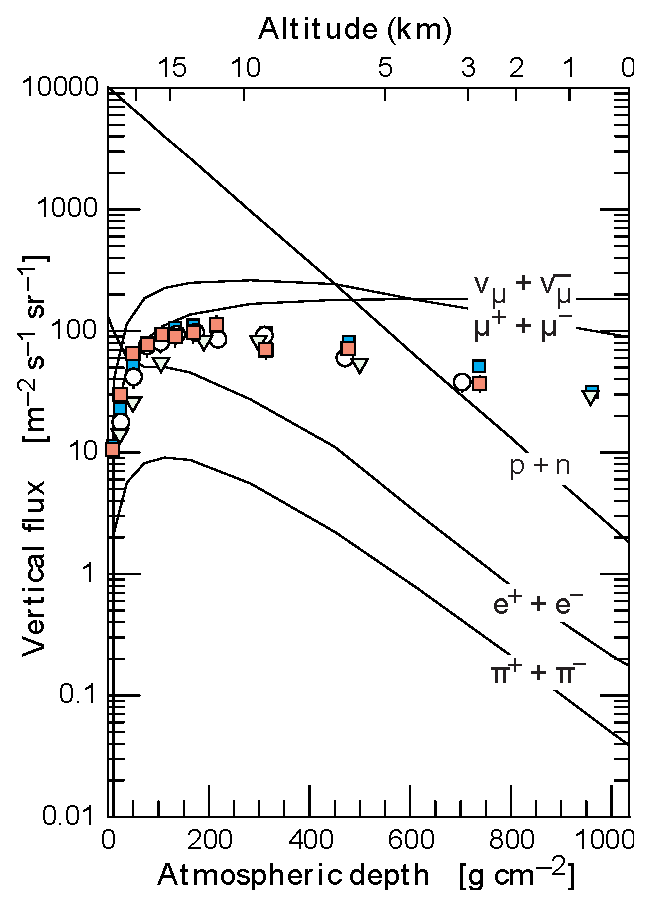
\includegraphics[width=.5\textwidth]{figures/chap2/atmospheric_cosmic_rays.eps}
	\caption[Estimated vertical fluxes of major cosmic ray components. Points are measurements of negative muons with energy larger than 1 GeV.]{Estimated vertical fluxes of major cosmic ray components. Points are measurements of negative muons with energy larger than 1 GeV.~\cite{Olive2014}}
	\label{figure:atmospheric_cosmic_rays}
\end{figure}

Daya Bay's experimental halls are also underground, and the muon-induced neutrons and isotopes constitute one of the major background sources. For Daya Bay, the sea-level muon energy and angular distribution is important because in order to get the energy and angular distribution in each hall with Monte Carlo simulation, the sea-level data, together with the mountain overburden profile and the rock composition, is input into the simulation and the muons are then propagated through the rock to get the propagated energy and angular distribution for those survived to the ceiling of the halls. Conventionally the sea-level muon flux is described by the Geisser formula~\cite{Beringer2012},
\begin{equation}
\frac{dN_\mu}{dE_\mu d\Omega}=\frac{0.14E_\mu^{-2.7}}{cm^2\cdot s \cdot sr \cdot GeV}\left\lbrace \frac{1}{1+\frac{1.1E_\mu\cos\theta}{115GeV}}+\frac{0.054}{1+\frac{1.1E_\mu\cos\theta}{850GeV}} \right\rbrace
\end{equation}
where the two terms in the braces give the contribution of pions and kaons, respectively.